\section{Analysis strategy}\label{chap6:AnalysisStrategy}

The analysis strategy for the first results on the high mass search in the $\mathrm{WW}\to2\ell2\nu$ decay channel closely follows the strategy presented in the 13\TeV Higgs boson measurement described in the previous chapter. In addition, a category dedicated to the VBF production mechanism is added, given the importance of this production mode in the high mass region. Indeed, assuming the production of a SM Higgs-like boson, the ratio of cross sections $\sigma_\mathrm{VBF}/\sigma_\mathrm{ggH}$ increases with the Higgs boson mass, making the VBF production mechanism more and more important as the mass of the resonance approaches to large values.

This analysis is essentially affected by the same background processes as the 125\GeV mass Higgs boson measurement, with the difference that in this case also the Higgs boson contribution is treated as background.

In addition to selecting events that pass the single or double lepton triggers, exactly one electron and one muon with opposite charges are required to be reconstructed in the event with a minimum \pt of 20\GeV for both the muon and electron. Both leptons are
required to be well identified and isolated to reject fake leptons and leptons
coming from in flight decays. To suppress background processes with three or more leptons in the final state, such as diboson or triboson production, events with any additional identified and isolated 
lepton with $\pt>10$\GeV are rejected. To suppress the contribution of the production of the Higgs boson at 125\GeV, \mll is requested to be higher than 50\GeV. The other event requirements are identical to the 125\GeV Higgs boson measurement and are described in Sec.~\ref{chap5:eventSel}.

In addition to the 0 and 1 jets categories, a specific category sensitive to the VBF production mode is defined exploiting the characteristic signature of this process, where two energetic jets are emitted in the forward region of the detector and are separated by a large $\Delta\eta$ region with a reduced particle density. Events belonging to the VBF-enriched category are selected by requiring at least two jets with $\pt>30$\GeV, an invariant mass $m_\mathrm{jj}>500$\GeV and a difference in pseudorapidity of $\Delta\eta_\mathrm{jj}>3.5$.

Beyond the transverse mass \mt, which is used in the analysis selection to define the \dytt background control region, an additional variable is defined, that from now on will be labelled as ``improved transverse mass'' \mti. This variable is defined as the invariant mass of the four momentum resulting from the sum of the two leptons four-momenta and the missing four-momentum $\mathbf{\MET} = (\MET, \ptmiss)$, i.e.:
\begin{equation} 
\mti = \sqrt{(p_{\ell\ell}+\MET)^2-(\vec{p}_{\ell\ell}+\ptmiss)^2} \quad .
\end{equation}

This variable allows a better sensitivity to different resonance mass hypotheses as illustrated in Fig.~\ref{fig:mti}, where the shape of the \mti variable is shown for different SM Higgs-like mass hypotheses and is compared to the standard \mt variable. The usage of this variable also provides a good discriminating power between signal and background.

\begin{figure}[htb]
\centering
\subfigure{
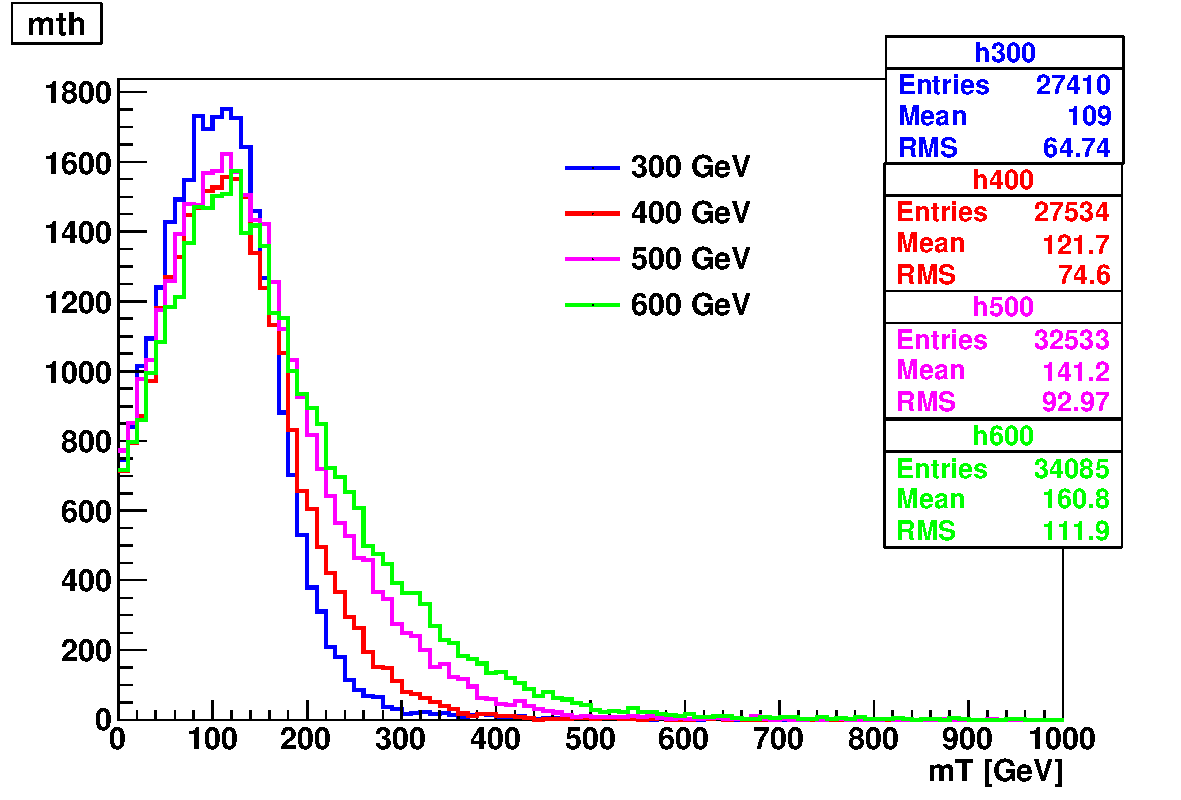
\includegraphics[width=0.45\textwidth]{images/13TeV/mT.pdf}
}
\subfigure{
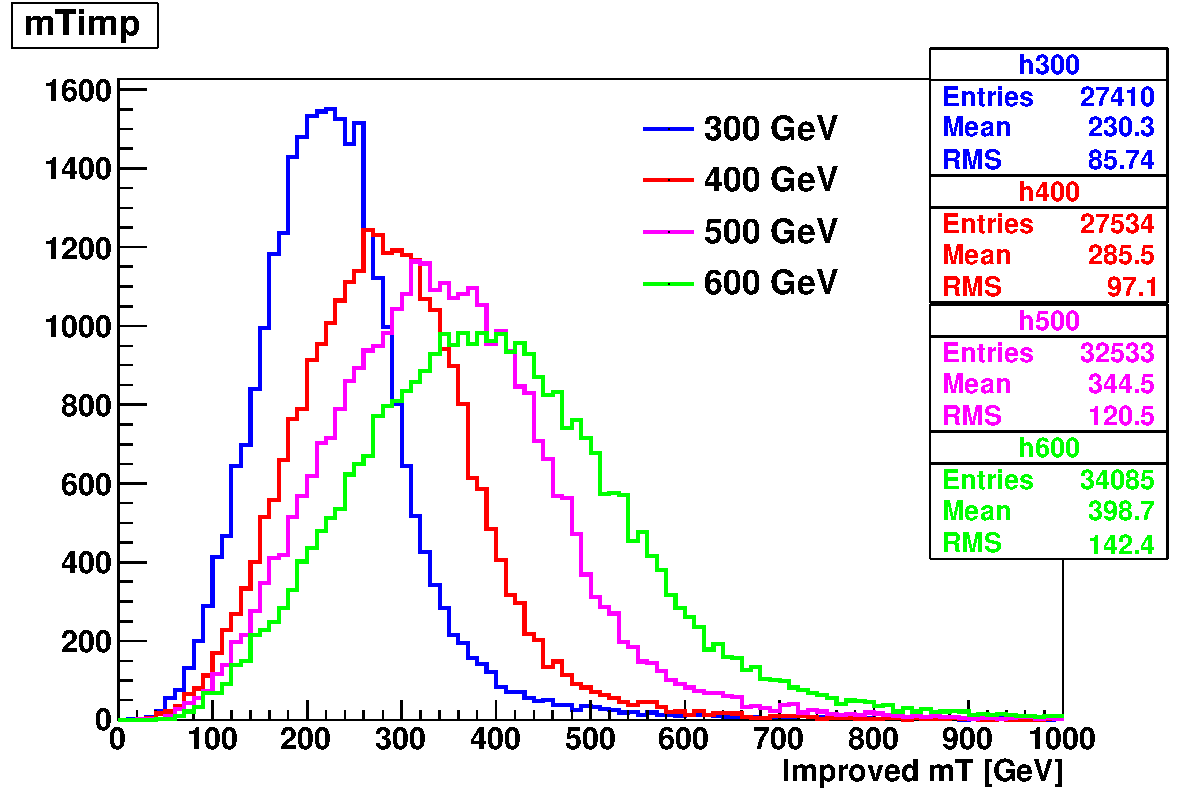
\includegraphics[width=0.45\textwidth]{images/13TeV/mTi.pdf}
}
\caption{
    Distributions of the \mt and \mti variables at generator level for different masses of the resonance.}
    \label{fig:mti}
\end{figure}

The signal extraction is based on a binned maximum likelihood fit using the \mti distribution for signal and background contributions as template. The \mti template is defined using the following bin boundaries:
\begin{itemize}
\item {0/1 jets: } [100,150,200,250,300,350,400,450,500,600,700,1000] ,
\item {VBF: } [100,150,200,250,300,350,400,500,700,1000] ,
\end{itemize}
where the first number represents the lower edge of the first bin while the other numbers represent the upper edges. The last bin is an overflow bin.

In order to test different resonance decay widths hypotheses, the signal samples, which are generated with a decay width corresponding to the expected value for a SM Higgs-like boson at that mass ($\Gamma_\mathrm{SM}$), are reweighted to obtain the desired width value ($\Gamma'$). In particular the following values are used: $\Gamma' = \Gamma_\mathrm{SM}$, $\Gamma' = 0.49 \times \Gamma_\mathrm{SM}$, $\Gamma' = 0.25 \times \Gamma_\mathrm{SM}$ and $\Gamma' = 0.09 \times \Gamma_\mathrm{SM}$.
The reweighting is performed at generator level by computing the ratio of two relativistic Breit Wigner distributions with different decay widths, $f(E,\Gamma',M_\mathrm{X})/f(E,\Gamma_\mathrm{SM},M_\mathrm{X})$, where:
\begin{equation}
f(E) \propto \frac{1}{(E^2 - M^2)^2 + M^2\Gamma^2} \quad .
\end{equation}
Here, $f(E,\Gamma_\mathrm{SM},M_\mathrm{X})$ represents the distribution used for simulating the signal at a mass $M_\mathrm{X}$, and $f(E,\Gamma',M_\mathrm{X})$ the distribution with the new decay width. Each event is multiplied by this ratio (which depends on the energy $E$ of the event) to obtain the reweighted distribution.

When a resonance with a non negligible width is considered, it is important to take into account the interference effects both with the gg$\to$WW background and with the off-shell tail of the 125\GeV Higgs boson.
A study of the interference effects for a resonance X produced through the gluon fusion mechanism is performed within the \textsc{MCFM}+\textsc{JHUGen} framework, including NNLO cross section corrections using the \textsc{HNNLO} program~\cite{Grazzini:2008tf}. The matrix element package MELA supports all these processes and allows fast MC reweighting and optimal discriminant calculation. The basic idea of this approach is to compute the matrix elements of the processes under study with the \textsc{MCFM} and \textsc{JHUGen} generators, including the interference terms, and using these matrix elements to compute an event weight used to reweight the simulated samples. Using this approach the simulated events can be reweighted according to different scenarios, for instance including some or all the interference terms, allowing a detailed study of the interference contribution. The effect of the various interference terms for the $M_\mathrm{X}$ variable at generator level is shown in Fig.~\ref{fig:int300}, after having applied the WW baseline selections. As can be observed, the contribution of the interference of the scalar resonance with the gg$\to$WW background and SM Higgs boson have opposite sign and partially cancel out. This cancellation effect is different for different resonance masses and depends on the event selection.
In particular, the interference term with the 125\GeV Higgs boson off-shell tail is positive for values below $M_\mathrm{X}$ while it turns negative above $M_\mathrm{X}$. The contribution of the interference with the gg$\to$WW background is instead characterized by an opposite sign lineshape, thus leading to a partial cancellation when considering the total interference.

\begin{figure}[htb]
\centering
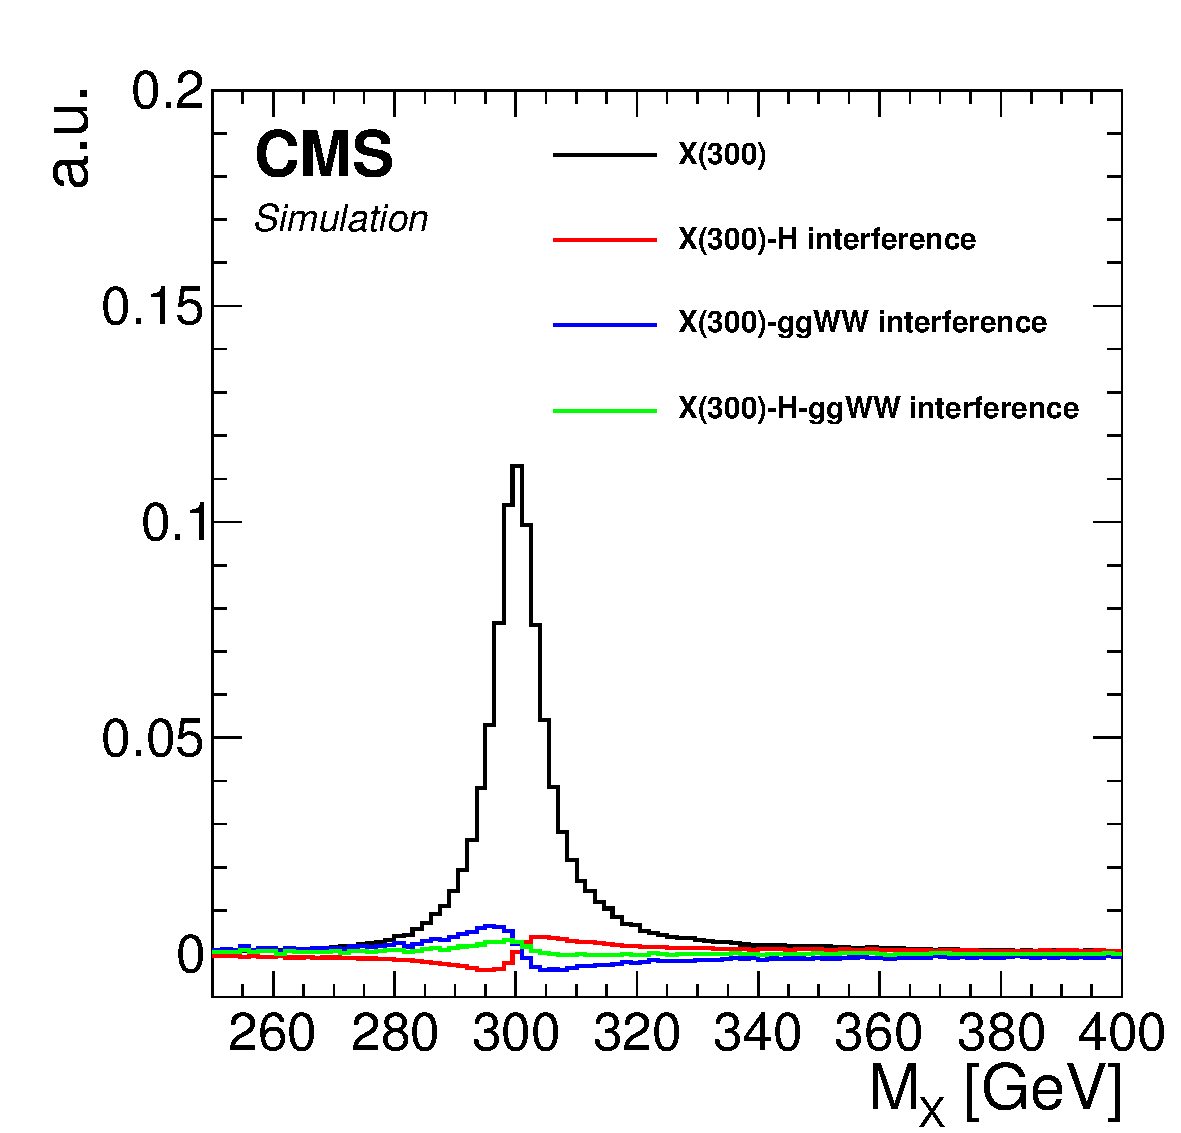
\includegraphics[width=0.7\textwidth]{images/13TeV/Interference/int300.pdf}
\caption{
    Distribution of the $M_\mathrm{X}$ variable for a resonance mass of 300\GeV, showing the various interference terms after the WW baseline selections.}
    \label{fig:int300}
\end{figure}

The effect of the resulting interference contribution including all the different terms is shown in Fig.~\ref{fig:mti_int} for the \mti signal templates, in the three categories separately and for different $M_\mathrm{X}$ hypotheses.

The interference contribution is thus not negligible, especially for large values of $M_\mathrm{X}$, and is included in the analysis as part of the signal process. More specifically, during the fit procedure the signal yield is scaled by the signal strength parameter $\mu$ (which is the parameter of interest of the fit), while the interference is scaled by $\sqrt{\mu}$.

\begin{figure}[!htb]
\centering
\subfigure[$M_\mathrm{X}=300$\GeV - 0 jets]{
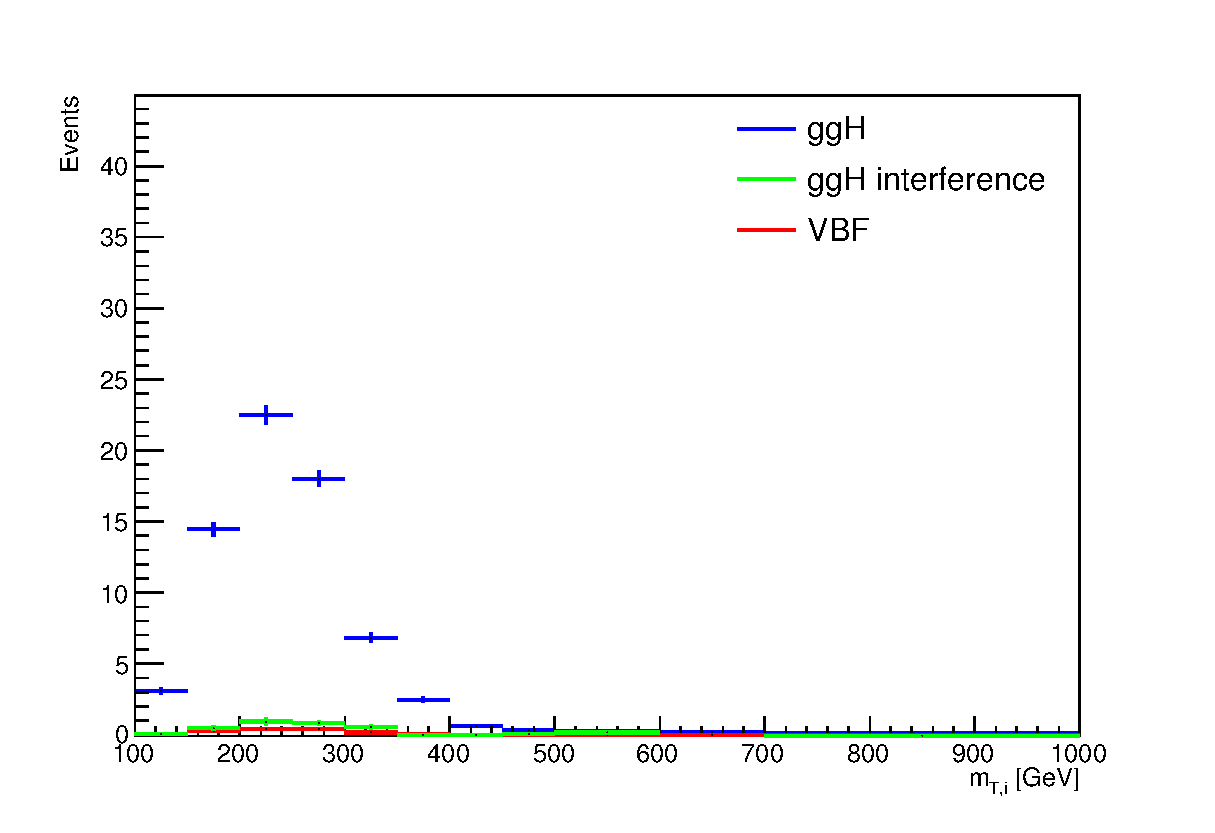
\includegraphics[width=0.4\textwidth]{images/13TeV/Interference/0j_300-v2.eps}
}
\subfigure[$M_\mathrm{X}=700$\GeV - 0 jets]{
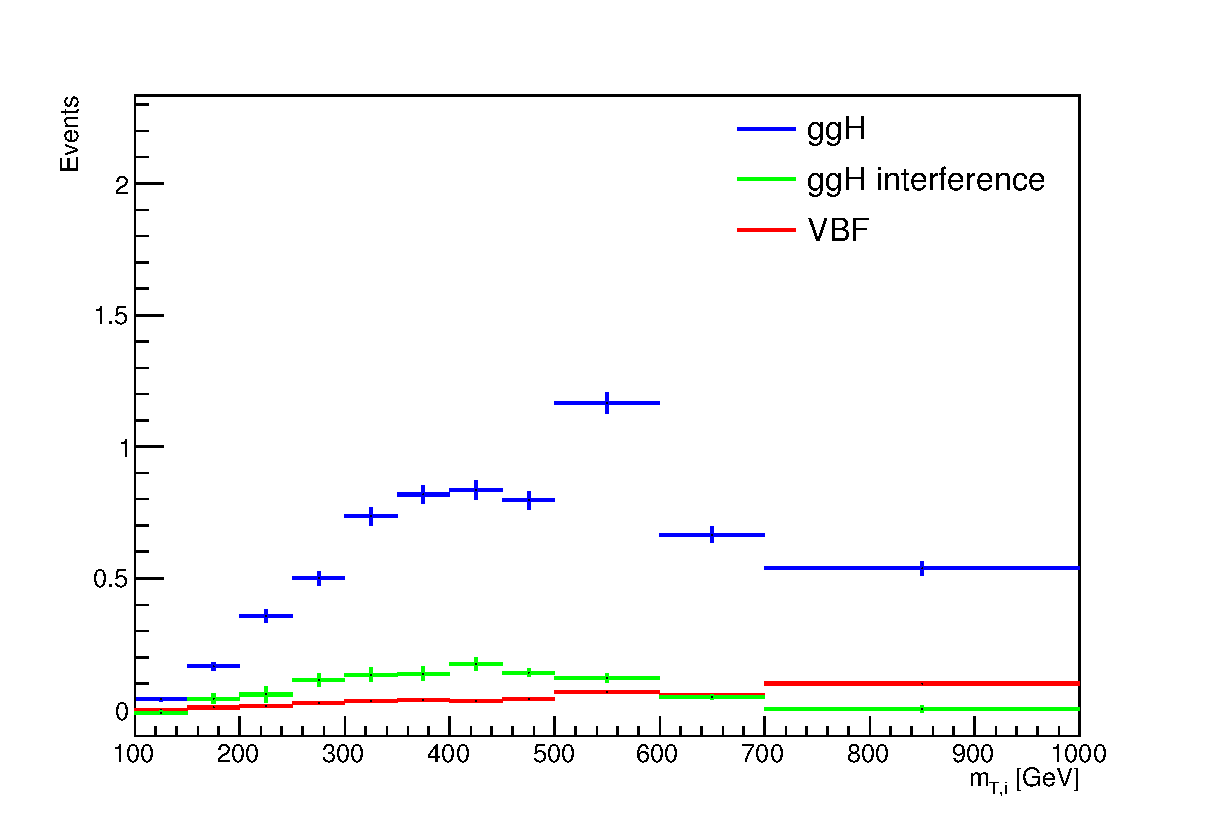
\includegraphics[width=0.4\textwidth]{images/13TeV/Interference/0j_700-v2.eps}
}\\

\subfigure[$M_\mathrm{X}=300$\GeV - 1 jet]{
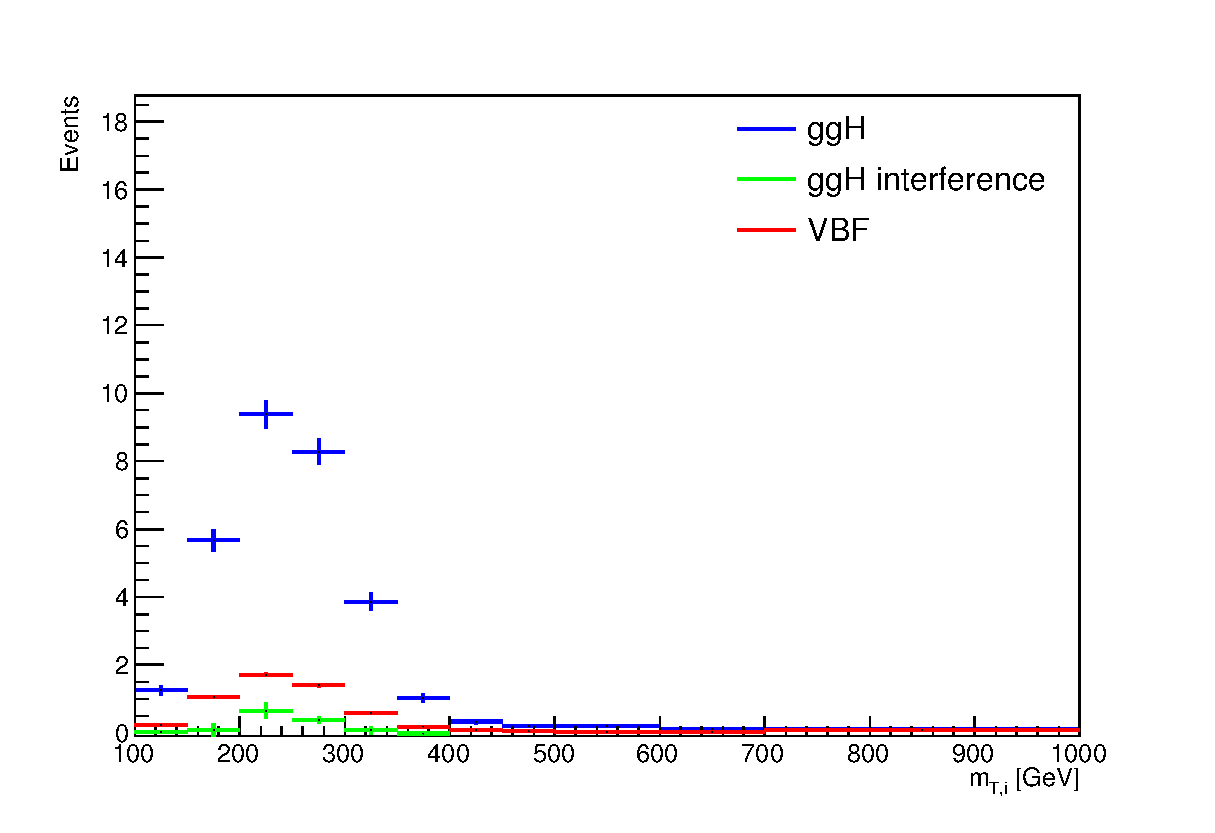
\includegraphics[width=0.4\textwidth]{images/13TeV/Interference/1j_300-v2.eps}
}
\subfigure[$M_\mathrm{X}=700$\GeV - 1 jet]{
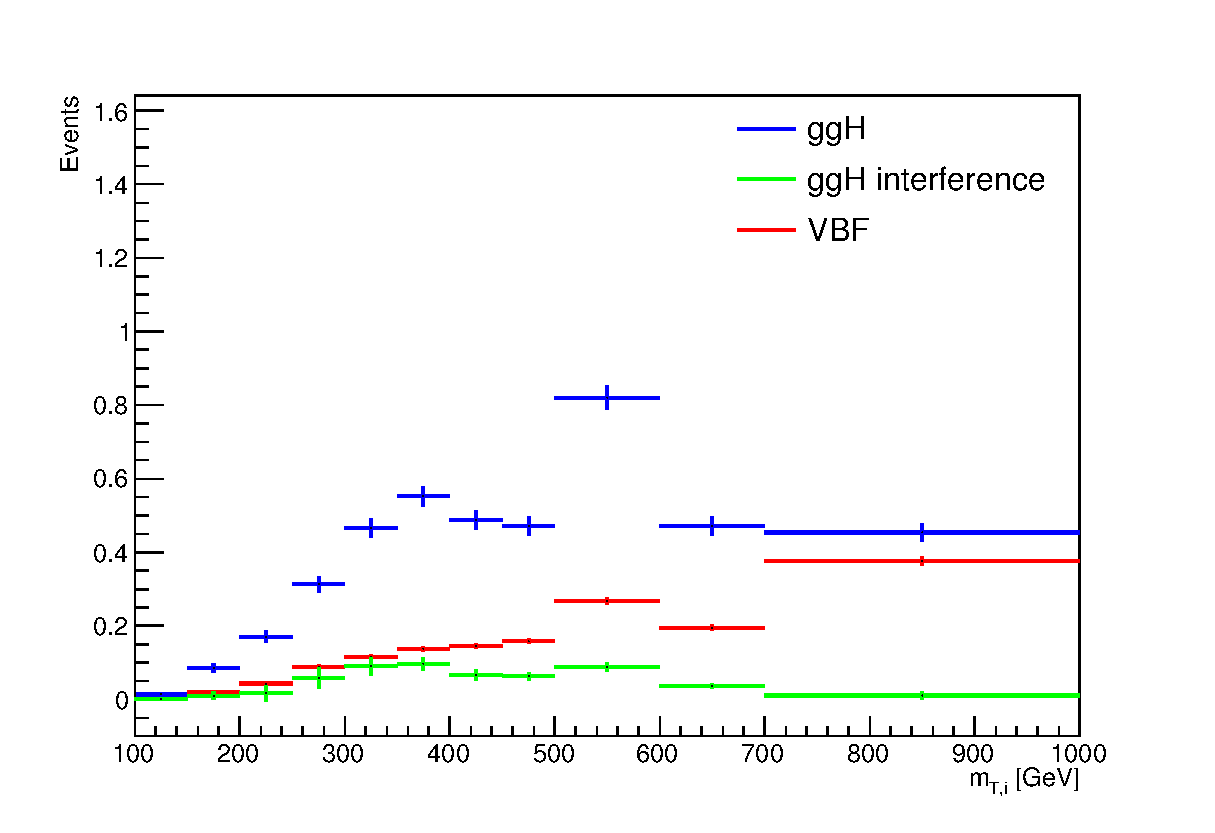
\includegraphics[width=0.4\textwidth]{images/13TeV/Interference/1j_700-v2.eps}
}\\

\subfigure[$M_\mathrm{X}=300$\GeV - VBF]{
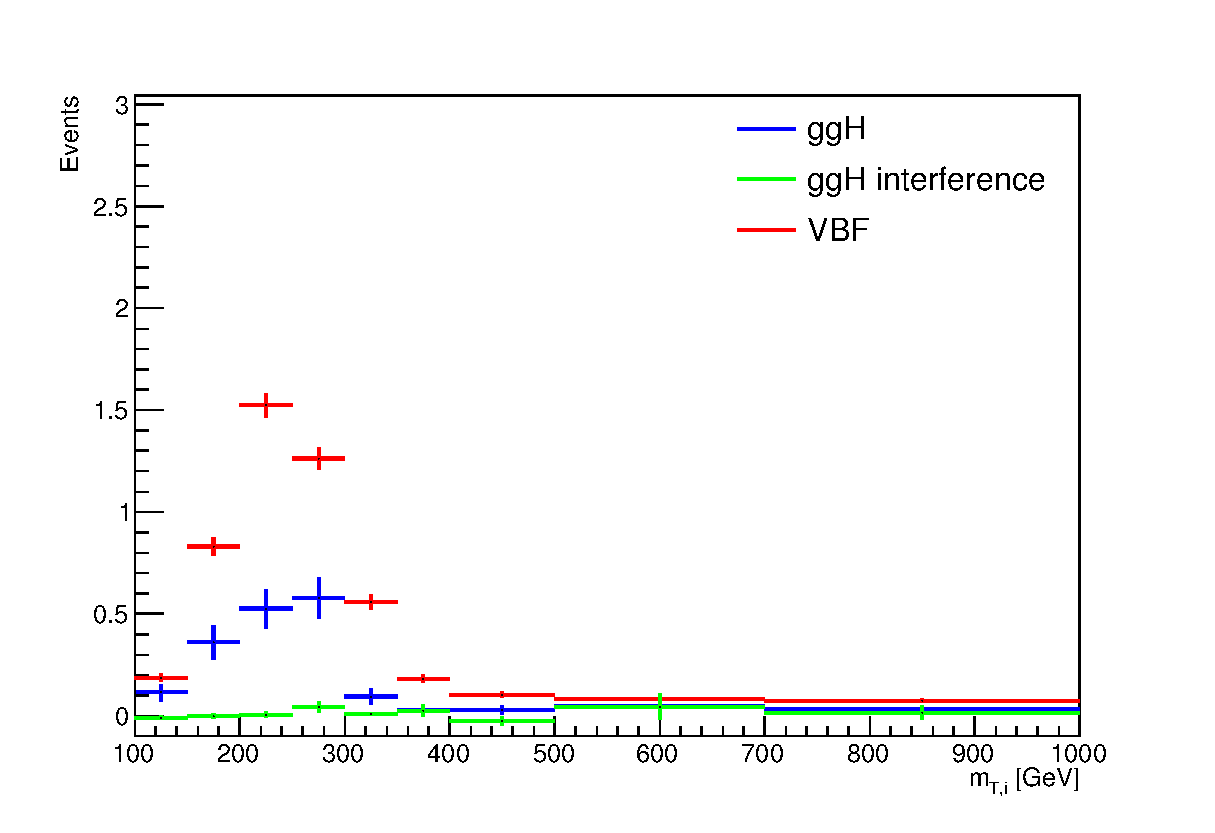
\includegraphics[width=0.4\textwidth]{images/13TeV/Interference/VBF_300-v2.eps}
}
\subfigure[$M_\mathrm{X}=700$\GeV - VBF]{
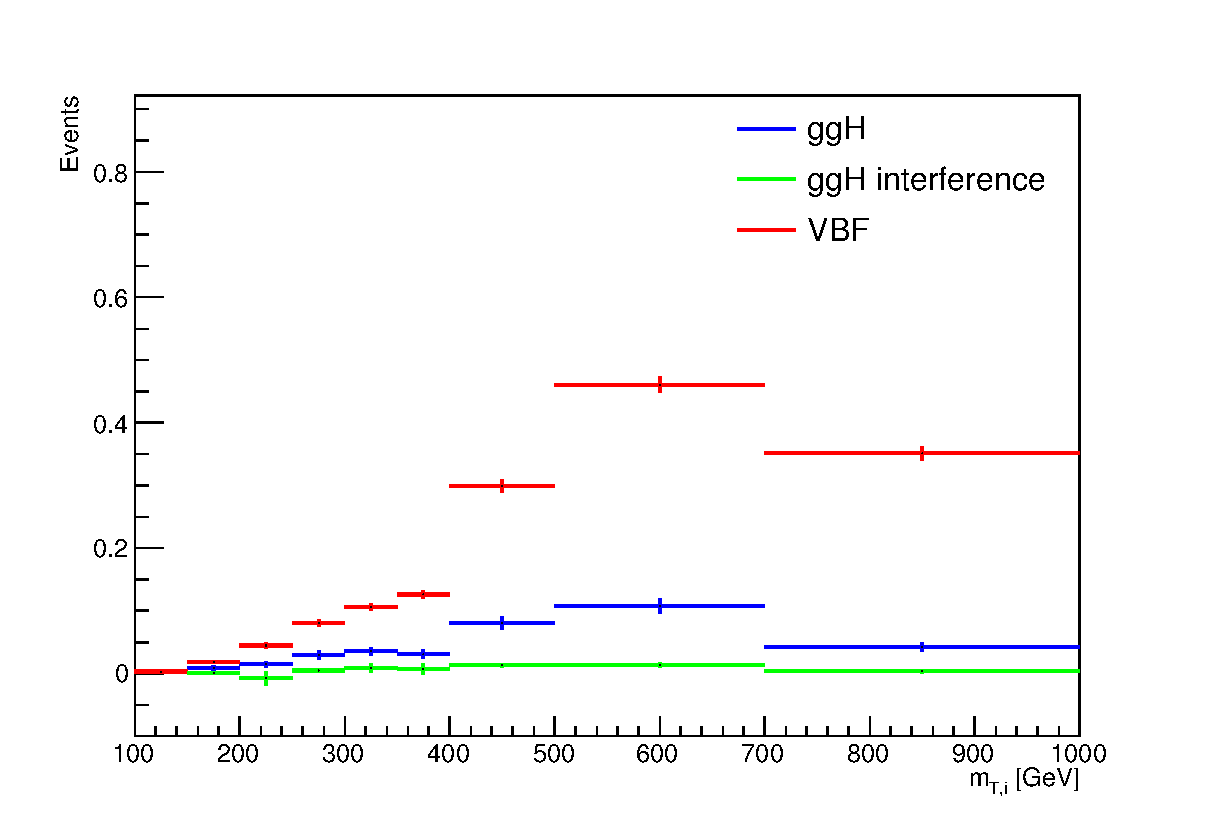
\includegraphics[width=0.4\textwidth]{images/13TeV/Interference/VBF_700-v2.eps}
}\\
\caption{
    Distributions of the \mti variable for $M_\mathrm{X}=300$ and 700\GeV, showing the signal (both the ggH and VBF mechanisms) and the interference contributions in the three jet categories.}
    \label{fig:mti_int}
\end{figure}


